\documentclass[conference]{IEEEtran}
\IEEEoverridecommandlockouts

\usepackage{cite}
\usepackage{amsmath,amssymb,amsfonts}
\usepackage{graphicx}
\usepackage{textcomp}
\usepackage{xcolor}
\usepackage{booktabs}
\usepackage{hyperref}

% ============================================================
% CA2 — H9MLAI Machine Learning
% Student: Alabi Taiwo Oluwatamilore | x24335592
% Due: 10 August 2026
% ============================================================

\begin{document}

\title{Automated Quality Assurance for AI-Generated Fashion Campaign Images:
Siamese Subject-Consistency Verification and Autoencoder Style-Drift Detection}

\author{
  \IEEEauthorblockN{Taiwo Alabi}
  \IEEEauthorblockA{
    MSc Artificial Intelligence \\
    National College of Ireland \\
    x24335592@student.ncirl.ie
  }
}

\maketitle

% ============================================================
\begin{abstract}
% 150–250 words. Standalone. State: problem / method / result / contribution.
% WRITE THIS LAST once you have real numbers.
% Template (fill in the blanks):
%
% Generative AI platforms such as kie.ai are increasingly used to produce
% commercial fashion campaign imagery at scale. Batch generation introduces
% two distinct consistency failures: subject-identity drift and grade-signature
% drift. This work implements and evaluates a two-component machine learning
% system to detect both failure modes. The primary component trains a Siamese
% network with a frozen ResNet50 backbone to classify image pairs as same-subject
% or different-subject. The secondary component trains a convolutional autoencoder
% on compliant images and uses reconstruction error as an unsupervised grade-drift
% signal. Both components are compared against a pixel-difference baseline and a
% k-Nearest Neighbours baseline over the same embedding space. The system is
% trained and evaluated on a curated dataset of [N] proprietary author-generated
% images from the Mullay fashion campaign pipeline. The Siamese network achieved
% F1=[___], outperforming the pixel-difference baseline (F1=[___]) and the kNN
% baseline (F1=[___]). The autoencoder correctly flagged [N] of [M] off-grade
% images with a reconstruction MSE threshold of [___]. These results demonstrate
% that metric learning on frozen convolutional embeddings provides a scalable,
% interpretable QA layer for AI-generated brand campaign imagery.
%
% ⚠ AI-DRAFTED SKELETON — REWRITE in your own words before submitting. Real
% numbers already filled from outputs/results/. Target 150--250 words.
Generative platforms such as kie.ai increasingly produce commercial
fashion-campaign imagery at scale, but batch generation introduces two
consistency failures: \emph{subject-identity drift}, where the generated person
stops being the contracted subject, and \emph{grade-signature drift}, where the
approved colour look departs. This paper implements and evaluates a
two-component machine-learning quality-assurance gate. The primary component is
a Siamese network with a frozen ResNet50 backbone that classifies image pairs as
same- or different-subject; the secondary component is a convolutional
autoencoder trained only on compliant imagery whose reconstruction error serves
as an unsupervised grade-drift signal. Both are benchmarked against a
pixel-difference baseline and a $k$-nearest-neighbour baseline over the same
embedding space, using a curated set of 106 proprietary author-generated images.
The Siamese network attained $F_1 = 0.90$ at perfect precision and
$\mathrm{ROC\text{-}AUC} = 1.0$, far exceeding the pixel-difference
($F_1 = 0.59$) and kNN ($F_1 = 0.26$) baselines, while the autoencoder flagged
62\% of synthetic off-grade probes at a 10\% false-alarm rate. The results show
that metric learning over frozen convolutional embeddings offers a scalable,
interpretable QA layer for AI-generated brand imagery.
\end{abstract}

\begin{IEEEkeywords}
Siamese networks, transfer learning, autoencoder, anomaly detection,
identity verification, generative AI, fashion imaging, quality assurance
\end{IEEEkeywords}

% ============================================================
\section{Introduction}
% ~400 words. Cover:
%  - The production context: Mullay campaign, kie.ai, batch generation
%  - The two failure modes (identity drift + grade drift) with evidence
%  - Why existing tools fail (face_recognition on synthetic faces)
%  - Your approach (Siamese + AE) and the baselines
%  - Paper structure ("Section II reviews related work...")

% ⚠ DRAFT from companion REPORT MAP (I. Introduction) — in my voice, polish before submitting.
This project sits inside a real production problem. The Mullay campaign pipeline
commissions fashion imagery from two commercial generators, FLUX-2 and
GPT-Image-2, through the kie.ai platform, and it does this in batches of twenty
to thirty images at a time. Batch generation breaks in two specific ways. The
first is \emph{subject-identity drift}: across a batch the generated person
slowly stops being the contracted subject. The second is \emph{grade-signature
drift}: the colour grade or overall look wanders away from the approved campaign
style. Both are expensive, because a single wrong-identity or off-grade asset
shipped to a client means a reshoot.

Right now the only real defence is a human screening every generated frame, and
that does not scale when the pipeline produces hundreds of images a day. The
obvious off-the-shelf fix, the \texttt{face\_recognition}/dlib library, was
tried early and failed: it is built for natural photographs and its distance
rule does not transfer to synthetic face textures.
% FIXME(research question): insert the RQ VERBATIM from docs/MARK_GUARD_CA2.txt
% (rubric row 1 needs it near-verbatim). You moved docs/ out -- paste it here.
\textbf{[Research question --- paste verbatim from MARK\_GUARD\_CA2.txt.]}

My approach is a post-hoc quality-assurance gate with two components. A Siamese
network with a frozen ResNet50 backbone answers the identity question (same
contracted subject, yes or no), and a convolutional autoencoder answers the
grade question (approved look, yes or no). Both are measured against two
deliberately simple baselines --- pixel difference and $k$-nearest neighbours
over the same embeddings --- so any gain has to be earned. The rest of the paper
is organised as follows: Section~\ref{sec:motivation} sets out the motivation,
Section~\ref{sec:related} reviews related work, Section~\ref{sec:method}
describes the methodology under the CRISP-DM stages, Section~\ref{sec:eval}
reports the evaluation and error analysis, and Section~\ref{sec:conc} concludes.

% ============================================================
\section{Motivation}
\label{sec:motivation}
% ~300 words. Expand on commercial impact:
%  - Client campaign requires consistent contracted subject
%  - False alarm rate of pixel-diff detector in practice
%  - face_recognition prototype failure: domain gap with synthetic textures
%  - Grade drift: four locked grade signatures, latent-space stochasticity

% ⚠ DRAFT from companion REPORT MAP (II. Motivation) — in my voice, polish before submitting.
The commercial case is simple. A client campaign is built around one contracted
subject, and every asset that ships has to be unmistakably that person in the
approved look. When identity or grade drifts, the asset is unusable, and
unusable assets mean reshoots --- the most expensive thing a campaign can hit.

This is why the two kinds of error are not equal for me. A missed detection ---
a wrong-identity image waved through the gate --- reaches the client and does
real damage, so recall on the ``same subject'' decision is the number I protect
first. A false alarm is cheap by comparison: it only triggers a re-generation,
which costs a few credits and a minute. The whole gate is therefore tuned around
the costly mistake, not the cheap one.

The naive fixes do not hold up. Pixel comparison collapses the moment the
subject turns their head, because a change of angle moves every pixel even when
it is the same person. The \texttt{face\_recognition} prototype looked
promising, but its 0.6 distance convention --- calibrated on natural
photographs --- was badly miscalibrated on my synthetic faces. And grade drift
cannot be caught by any identity tool at all: it is a separate failure that
needs its own detector, which is why the system carries a second, unsupervised
guard.

% ============================================================
\section{Related Work}
\label{sec:related}
% ~500 words. Cite all 7+ papers. End with the gap statement.
%
% Subsections (optional):
%   A. Siamese Networks and Metric Learning
%   B. Identity Consistency in Generative Models
%   C. Style Consistency and Anomaly Detection
%   D. Research Gap

% ⚠ DRAFT from companion REPORT MAP (III. Related Work) — in my voice, cites all 9, polish before submitting.
My identity check builds on metric learning: training a network to measure how
similar two images are, rather than to name a fixed set of classes. Chopra et
al.\ introduced the contrastive framework for exactly this face-verification
setting~\cite{chopra2005contrastive}, and Koch et al.\ showed a Siamese network
can verify identity from very few examples per class~\cite{koch2015siamese} ---
the one-shot property that matters when, like me, you have only two subjects.
Schroff et al.'s FaceNet~\cite{schroff2015facenet} is where the
128-dimensional L2-normalised embedding I use comes from. All of these sit on a
convolutional backbone; I use ResNet50~\cite{he2016resnet}, whose residual
design keeps deep feature extraction stable and which, pretrained on ImageNet,
gives a strong off-the-shelf encoder.

The reason this problem exists at all is the recent wave of subject-driven image
generation. DreamBooth~\cite{ruiz2023dreambooth} and
InstantID~\cite{wang2024instantid} can lock a specific person's identity into
generated images, and attention-sharing methods like
Prompt-to-Prompt~\cite{hertz2022prompt} control how the look is edited between
generations. These tools are what make campaign-scale synthesis possible --- but
they are generators, not verifiers. None of them checks its own output after the
fact.

For the grade side I borrow from anomaly detection, where a model learns only
the normal case and flags deviation. Chalapathy and Chawla survey the
deep-learning approaches~\cite{chalapathy2019deep}, and Bergmann et al.'s MVTec
work~\cite{bergmann2019mvtec} shows that reconstruction error from a model
trained only on good examples is a reliable industrial defect signal --- exactly
the mechanism my autoencoder uses.

The gap is the combination. Plenty of work generates identity-consistent images,
and plenty detects anomalies, but none of the reviewed work puts a post-hoc gate
that checks \emph{both} subject identity \emph{and} grade compliance on
AI-generated fashion imagery. That combined QA layer is what this project builds.

% ============================================================
\section{Methodology}
\label{sec:method}
% CRISP-DM structure per rubric row 4: Business Understanding -> Data
% Understanding -> Data Preparation -> Modelling -> Evaluation Protocol ->
% Deployment. Your own written content arranged under the stage names the
% marker scans for.

\subsection{Business Understanding}
The Mullay campaign pipeline commissions fashion imagery from two commercial
text-and-image generation models (FLUX-2 and GPT-Image-2) through the kie.ai
platform. A campaign requires many styled shots of the \emph{same} contracted
subject across poses, outfits and camera angles. Batch generation introduces
two distinct, commercially costly failure modes: \emph{subject-identity drift}; this is
where the generated person gradually stops being the contracted subject, and
\emph{grade-signature drift}, where the colour grade or look departs from the
approved campaign style. The business goal is therefore an automated QA gate: given a newly
generated image, accept it into the campaign only if it (i) depicts the
contracted subject and (ii) carries the approved grade.

\subsection{Data Understanding}

\subsubsection{The Dataset, Counted Properly (what pair\_builder actually eats)}
% FIXME (your call): the subject appearance sentences below read informal for an
% IEEE report ("covered in some moist", "small beard above her upper lip") —
% earlier review suggested cutting or neutral phrasing. Left verbatim per your
% instruction.
There are two subjects; subject A and subject B. Subject A is a photo of a young aged man, some freckles covered round his face, as well as what appears to be a well moisturized hair.
Subject B is a photo of a young woman, who seems to be a bit covered in some moist, subject B is interesting, because she seems to have a small beard, above her upper lip. Each subject has a styled folder, with exactly 50 images. Where the 50 comes from: for every angle I generated 5 samples with flux-2 image-to-image generator, and 5 samples with gpt-image-2, so 10 images per angle. There are 5 angles, named: (3qleft, 3qright, profileleft, profileright, back).
The multiplier comes from the n samples generated per angle from both gpt-2 and flux-2.

Each subject also has 3 reference images sitting at the top of \texttt{hero\_ref/}: the original pinterest photo (new\_hero), the flux-2 hero front (hero\_front\_flux2test), and the gpt-2 hero front (hero\_front\_gpt2test). This makes the real identity anchor not one, but three.

Full count per subject: 3 reference/id photos + 50 styled = 53 images. Both subjects together: 106 images. That is everything pair\_builder.py reads.

How 106 images become 600 pairs: positives are every ref x every styled of the SAME subject: 3 x 50 = 150 per subject, 300 total, label 1. Negatives are every ref x every styled of the OTHER subject: 3 x 50 crossed both ways = 300 total, this makes total 600 pairs. This in pairs\_manifest.json.

% FIXME(grades removed, factual): this "teal vs dark grades" cheat example uses colour
% grades that do NOT exist in your data. Swap it for the REAL anti-cheat argument you
% already make in "Both Models Feed the Dataset" below: matching the two GENERATORS
% (flux-2 AND gpt-2) across both subjects is what forces identity learning, not colour.
% <<< REWRITE this sentence in your own words using the generator argument >>>
To explain further; negatives pair different people generated the SAME way (both generators, both subjects). The point is that matching the shared factors across subjects leaves identity as the only signal the network can learn.

\begin{table}[h]
\caption{Dataset Summary}
\label{tab:dataset}
\centering
\begin{tabular}{lc}
\toprule
\textbf{Property} & \textbf{Value} \\
\midrule
Total images & 106 \\
Subjects & 2 \\
Hero references per subject & 3 \\
Styled shots per subject & 50 (5 angles $\times$ 10) \\
Generation models & 2 (FLUX-2, GPT-Image-2) \\
Total pairs & 600 \\
Positive / negative pairs & 300 / 300 \\
Train / Val / Test pairs & 420 / 90 / 90 (70/15/15\%) \\
\bottomrule
\end{tabular}
\end{table}

\subsubsection{Both Models Feed the Dataset (why each angle has 10 images)}
Important detail I want to state clearly: I did not pick one winning model and throw the other away. Every angle folder holds shots from BOTH generators, images 1 to 5 are flux-2's five tries, images 6 to 10 are gpt-image-2's five tries. That is what makes it 10 per angle. The Siamese network trained on images from two different generators at once. So when it says 'same person', it learned to recognise identity across flux-2's rendering look AND gpt-2's rendering look, not just one models style. It also blocks another cheat. If subject A only existed in flux-2 images and subject B only in gpt-2 images, the network could learn 'flux-2 texture = A' without ever reading a face
Same trick as the grade-matching, match the grades across subjects, match the generators across subjects, and the only signal left for the network to learn is the face itself.

\subsection{Data Preparation}
% ⚠ AI-DRAFTED SKELETON PARAGRAPH — integrity rule for H9MLAI says AI may not
% write submission content. REWRITE this stage in your own words before
% submitting (facts to keep: seeded JSON manifest, stratified 70/15/15 split,
% 224x224 + ImageNet preprocessing, flip + ±10% brightness augmentation on
% train split ONLY, brightness kept small so it can't fake a grade drift).
Pairs are sampled and shuffled with a seeded generator and persisted to a JSON
manifest, so the dataset composition is itself an auditable artefact. The
70/15/15 train/validation/test split is stratified by class: positive and
negative pairs are permuted and partitioned separately with a seeded NumPy
generator, preserving the 50/50 class balance in every split (420/90/90
pairs). Each image is resized to $224 \times 224$ and normalised with the
standard ResNet50 ImageNet preprocessing~\cite{he2016resnet}. Light
augmentation --- a horizontal mirror flip with probability 0.5 and a
brightness perturbation of at most $\pm 10\%$ --- is applied to the training
split \emph{only}; validation and test images are never augmented, to avoid
data leakage. The brightness range is deliberately small so that augmentation
cannot alter the grade signature the second model is meant to detect.

\subsection{Modelling}

\subsubsection{Where ResNet50 and ImageNet Come Into My Pipeline}
Up to now the story was: generate images, apply styles, build positive and negative pairs. Here is where they fit and what they actually are, ImageNet is a giant public dataset of about a million labelled photos (objects, animals, people), released by Stanford researchers. ResNet50 is a neural network that was trained on all of it. Think of a doctor who trained for years on a million real scans, she has already learned how to SEE. That is ResNet50.
This is transfer learning: instead of teaching a network to see from scratch using only my 106 images (impossible - too few), I borrow a network that already learned to see from a million images and apply it to mine.
What ResNet50 does with one of my photos?
It does not store it or memorise it. It reads the photo and outputs a fingerprint - a list of 2048 numbers describing what it sees (face shape, skin texture, eye spacing, and so on). That fingerprint is called an embedding. Two photos of the same woman get very similar fingerprints; two different women get different ones.
Frozen means: I never re-train ResNet50. Its weights stay exactly as ImageNet left them. My
two reasons for these are; One, my 600 pairs cannot compete with a million training images, retraining would make it worse, not better. Two, freezing keeps the Siamese network's job small and honest: it only has to learn how to compare two fingerprints, not how to see.
The 224 x 224 rule, ResNet50 was trained with every ImageNet photo resized to 224 x 224 pixels and colour-shifted by fixed ImageNet mean values. So every one of my images must be served exactly the same way, or the fingerprints mean nothing.
% FIXME (factual, per backbone.py:50-56): the flow below skips the trainable
% Dense funnel that squeezes 2048 -> 128 before the L1 comparison. As written
% it contradicts the 128-number description in "How Siamese Works". Add the
% funnel step in your own words.
The full flow, start to end: my 106 raw images (all sizes) $\rightarrow$ preprocessing.py resizes to 224x224 and applies the ImageNet colour shift $\rightarrow$ frozen ResNet50 turns each into a 2048-number fingerprint $\rightarrow$ the Siamese head takes two fingerprints, measures the L1 distance between them, and outputs one number from 0 to 1: same person or not.
The consistency point: because the same frozen network reads every image through the same preparation, every comparison is fair. Nothing is stored, nothing drifts between runs - the backbone is a fixed measuring instrument.

\subsubsection{How Siamese Works}
% FIXME (dangling sentence): "used twice" — say the two uses (training + QA
% gate at deployment) or a marker will ask.
The Siamese network is used twice.
The architecture is as follows,
photo A $\rightarrow$ same frozen ResNet50 $\rightarrow$ two 128-number fingerprints
photo B $\rightarrow$ L1 distance (compute the 128 absolute differences) $\rightarrow$ Dense(1, sigmoid) (the only layer that learns) $\rightarrow$ one number: 0.0 to 1.0 (probability of same person).
% FIXME (factual, per backbone.py:48 + siamese.py): "the only layer that
% learns" is not what the code does — the Dense 2048->128 funnel ALSO trains
% (only the ResNet50 base is frozen; 262,401 trainable params ~1% of network).
% Same issue where it repeats two paragraphs down and in the next subsection.
The L1Distance layer: takes two fingerprints, subtracts them (emb\_a - emb\_b), and drops the minus signs (absolute value). The result is a list of 128 differences. Same person fingerprints produce mostly tiny differences. Different people produce many big differences.
The Dense(1, sigmoid) layer: this is the only layer that learns during training. It takes the 128 differences and asks: which of these 128 dimensions actually matter for telling people apart? Which are just noise? During training, it learned to weight the important dimensions and ignore the noisy ones. \textbf{That is why it beats the baselines}.
% FIXME (placement): the sentence above + the "Why this wins" sentence below
% state RESULTS inside Methodology — earlier review advised phrasing as design
% rationale here and proving it in the Evaluation section.
Why this wins over the baselines, pixel-difference just measured pixels directly and failed when angles changed. kNN used all 128 dimensions equally, treating noise the same as signal. Siamese's Dense layer is smarter, it learned which dimensions matter.
Training: Adam optimizer with learning\_rate=1e-4 (careful small steps). Binary cross-entropy loss (if it says 0.9 but the answer is 1.0, penalize heavily). Metrics tracked: precision, recall, ROC-AUC (the rubric scorecard).

\subsubsection{Understanding siamese.py (every design knob, explained)}
Why 1: Only 1 layer learns, not multiple?
If we unfroze ResNet50 and let multiple layers learn, we'd need a million images to re-train it. We only have 600 pairs. So: freeze the expert, train only the decision layer on top. We applied transfer learning = keep the old knowledge frozen, add one small trainable head.
My choice of optimizer is; Adam optimizer, not SGD or RMSprop. Adam is the modern standard because it adapts per-dimension, some of the 128 fingerprint dimensions might be 'steep' and need tiny steps; others are 'flat' and can handle bigger steps. Adam handles both. For the learning rate 1e-4 is Goldilocks: careful enough not to break the frozen ResNet50 features, fast enough to converge in $\sim$11 epochs.
Loss function is Binary Cross-Entropy. If the model says 0.9 but it was 0 (certain it's the same person, but it was different)? That's confidently wrong. Big punishment. Its perfect for this 2-class problem (same/different, 1/0, yes/no)
% FIXME (placement): the results sentence below (precision 1.0 / recall 0.82)
% belongs in the Evaluation section's Results, not in Methodology.
My Siamese: precision = 1.0 = it never raised a false alarm. Perfect. My Siamese: recall = 0.82 = it caught 82\% of same-person pairs. Good, but not perfect because those 8 were really hard angles.

\subsubsection{Why kNN Cannot Cancel Noise (and Siamese can)}

My question was: can't the sigmoid function cancel off noise in kNN too? Answer: no, because kNN has no sigmoid and nothing that learns. That is the entire difference between the two models.

kNN takes the raw ResNet fingerprints and measures plain distance, every dimension counts equally. Noise dimension \#93 (say, background tint) votes with the same power as jawline dimension \#7. Nobody ever taught kNN which votes to trust. It cannot cancel noise because it has no trainable weights.

The Siamese Dense(1, sigmoid) layer has 128 learnable weights, one per dimension. During training, every mistake pushes the weight on noisy dimensions toward zero and grows the weight on identity dimensions. The sigmoid itself does not cancel the noise, it just squashes the final sum into 0-1. The weights before the sigmoid do the cancelling.

The build\_siamese\_model() assembles the machine (ResNet50 lives inside it as the two frozen arms, plus L1Distance, plus the Dense sigmoid head). compile() sets the knobs on the machine. (which tutor = Adam, which punishment rule = binary cross-entropy, which scorecard = precision,recall, as well as ROC-AUC), no training happens at compile. fit() is the actual cooking, it is where the Dense layer learns. build = assembles, compile = sets the knobs, fit = train.

kNN weighs all embedding dimensions equally, whereas the Siamese head learns per-dimension weights, effectively learning which features carry identity.

% ⚠ AI-DRAFTED SKELETON PARAGRAPH — rubric wants BOTH baselines described with
% hyperparameters (pixel-diff threshold 0.05; kNN k=5 vestigial, distance
% threshold 0.6). Your kNN subsection above covers the "why"; this paragraph
% still holds the pixel-diff numbers. REWRITE in your own words, then delete.
\paragraph{Baselines}
Two baselines bound the problem from below. \emph{Pixel difference} computes
the normalised mean-squared pixel error between the raw $224 \times 224$
images and predicts ``same subject'' below a fixed threshold of 0.05; it
represents naive template matching and is expected to fail whenever pose or
angle changes, since a head turn moves every pixel. \emph{kNN over
embeddings} ($k=5$) reuses the identical frozen ResNet50 embedding space as
the Siamese network but does not learn a decision boundary: it predicts
``same subject'' when the Euclidean distance between embeddings falls below
0.6, the conventional \texttt{face\_recognition} threshold. This isolates the
contribution of the \emph{learned} comparison head: any gap between kNN and
the Siamese network is attributable to learning, not to the representation.
The distance threshold, not $k$, is the operative hyperparameter of this
baseline, and it is swept in Section~\ref{sec:eval}.

\subsubsection{The Autoencoder (the second guard: grade drift, not identity)}
My QA system has two checks, not one. The siamese asks; is this the same person? (identity check). The autoencoder asks: does this image have the right look or style? (grade check). An image can pass one and fail the other, for example, right woman but washed-out colours means Siamese passes it and the autoencoder catches it.
% FIXME(grades removed, factual): the 4 named colour grades (teal_orange/warm_portra/
% dark_moody/triX_street) were NEVER generated -- they do NOT exist in data/. The AE
% actually trains on the compliant styled campaign images (both subjects); the "off-grade"
% test images are SYNTHETIC distortions made at runtime in run_parametrisation_experiments.py
% Exp 4.3: hue-shift (+60deg), overexposure (brightness x1.8), desaturation (colour x0.1).
% <<< REWRITE the sentence below in your own words to say exactly that >>>
The autoencoder is shown only correct, compliant campaign images (the styled shots of both subjects). Then the test is, look ath this image for one second, now redraw it from memory. A normal image the autoencoder has seen a thousand times, will be redrawn nearly perfect, with perhaps a tiny error. Compared to, an
off-grade image (over-exposed or hue-shifted) the machine has never seen anything like it, the redraw comes out wrong, Big error here. The redraw error here is the alarm. Never saw a single bad example, yet detects bad, by failing to redraw it. That is why it is called unsupervised: no labels needed, only normal images.
Why the autoencoder cannot cheat?
% FIXME (factual, per autoencoder.py): the chain below reads as "image 64 ->
% 32 -> 16 -> 64" — the actual encoder is three conv blocks (32, 64, 128
% filters) with 2x max-pooling shrinking the image 128 -> 64 -> 32 -> 16,
% then the dense bottleneck of 64. Restate in your own words so the numbers
% match the code.
The image is 128x128x3 = 49,152 numbers, but it must squeeze through a memory of only 64 numbers, then be redrawn from those 64. The encoder(squeeze): image  64 $\rightarrow$ 32 $\rightarrow$ 16 $\rightarrow$ just 64 numbers, and then the decoder (redraws): 64 numbers $\rightarrow$ 16 $\rightarrow$ 32 $\rightarrow$ 64 $\rightarrow$ full image again. Memorising pixels is impossible, the autoencoder can only keep the essence of the normal ( the grades color mood, lightning). Normal images survive the squeeze; weird images lose exactly the parts that made them weird.

The three functions in the file: build\_autoencoder() builds (encoder + decoder together). compile\_autoencoder() sets the knobs: Adam tutor, MSE loss (predicting pixels. reconstruction\_error() is the scoring bench: original minus redraw, squared, averaged. There will be one error number per image.

During training, the redraw errors are measured on normal images and a line at the 95th percentile will be drawn on those errors.(worse than 95\% of normal errors = suspicious). Any new image above that line, this confirms grade drift, the image fails Campaign Quality Assurance. My Experiment 4.3 showed the 90th percentile is actually the better dial, it catches 62\% of drifted images at 10\% false alarms.

% FIXME (stale cross-ref): "Section 1.2" below no longer exists after the
% CRISP-DM re-arrangement — point it at the design-knobs subsection name.
Key difference from siamese.py: There is no ResNet here. This little network trains from scratch - it does not need to learn how see the world, it only needs to learn 4 colour styles. That is also why its learning rate is 1e-3 (bigger steps) while Siamese used 1e-4 (frozen backbone = careful steps). The two files follow my own rule from Section 1.2.

\subsubsection{train\_siamese.py (the school term: fit, epochs, and the four supervisors)}

% FIXME (units, per train_siamese.py): trained on 420 PAIRS not images, and
% the mini-test is on 90 validation PAIRS. Also "Batch of 16 images shown 16
% at a time" doubles up — batch means 16 pairs at a time.
The network is trained on 420 images. Batch of 16 images shown 16 at a time, then the Adam optimizer adjusts the weights. After each epoch there is a mini-test on the 90 images. The file evaluate.py runs this.

The CONFIG file; all the knobs in one dict at the top (embedding 128, learning rate 1e-4, batch 16, max 50 epochs, save path). One dict so I can change one number without having to read through code - my Experiment 4.4 reused exactly this to retrain at dim 64 and 256.
The 4 callbacks, logging training activities are:
1. EarlyStopping - if there is no improvement in val\_roc\_auc for 10 days? epoch is over. And restore\_best\_weights=True means: go back to the brain you had on your best day, not your last day. This is the anti-overfitting guard, it stopped at epoch 11 of 50, saving approx. 80\% of my compute.

2. ModelCheckpoint - every time the validation record is broken, snapshot the brain to siamese\_best.keras.

3. ReduceLROnPlateau - if the validation loss is stuck for 5 days, take smaller steps,as per half the learning rate (1e-4, down to 5e-5 etc). Careful steps near the end.

4. CSVLogger - this is every day's scores written to siamese\_train\_log.csv.

Why monitor val\_roc\_auc and not train accuracy or val\_loss?
ROC-AUC asks a cutoff-free question instead: "if I hand you one same-person pair and one different-person pair, does the model score the same-person pair higher? AUC is the fraction of times it gets that ordering right. 1.0 = every genuine pair ranks above every impostor pair, perfect ranking, no cutoff involved.

Why that's the thing I actually care about: this deployment is a Quality Assurance gate whose threshold can move (stricter for a big client, looser for drafts). A model with perfect ranking stays good at every threshold you might pick. A model with good accuracy at say 0.5 might collapse the moment you move the cutoff.

Validation keeps the score honest; ROC-AUC keeps it honest at every possible cutoff, not just the one I happened to try.

\subsubsection{train\_autoencoder.py (the homework is the answer sheet)}
In siamese every photo pair had an answer on the back (1 or 0). Here there are no answers at all. The strangest line in the entire file is fit(images, THE SAME images). The autoencoders homework here is, here is a photo, redraw it from the original. Pixels are divided by 255 because the decoder ends in a sigmoid that can only output 0-1
the prep must match what the output layer can draw. There is a 80/20 train/val split with no test stack, the real test came later in Experiment 4.3 with synthetic bad images (hue shift and overexposure). It monitors val\_loss not val\_roc\_auc, so there is no ranking of classes here, the only score is redraw error. There is a total of 106 images, the train/validation split is 85/21, i set the max epochs to 100, it is worth noting validation loss; val\_loss stopped improving around $\sim$52, just to be sure, it continued for another 15 epochs, then ended total epochs at 67 and restored best weights. So up to 100 was the total budget; 67 was the spend. Batch size is set to 8.

% FIXME (number, per outputs/results/ae_threshold.json): threshold_mse is
% 0.005033 (train mean 0.004021 ± 0.00066) — "MSE 0.004259" below matches
% neither. Re-check where 0.004259 came from before submitting.
The extra step siamese never had. Measure the redraw error on every good training image, line the errors up, put the line at the 95th percentile so that a worse than 95\% of your normal work becomes suspicious. Mine landed at MSE 0.004259, saved with its stats to ae\_threshold.json. The threshold is learned from data, not invented or configured.

The Siamese (with its million-image frozen expert) needed only 11 epochs; the autoencoder (learning to see from scratch) needed 67. Both finished in under a minute, 371s vs 49s, but the epoch count tells the transfer-learning story in one comparison: borrowed eyes converge 6x faster than eyes grown from zero.

\subsection{Evaluation Protocol}

\subsubsection{evaluate.py (exam day: one marker, three students)}
The 90 test images have been sealed since preprocessing.py handled them. Now Siamese, pixel-diff, and kNN sit the exam. All three will be graded with the same rubric. If each model measured itself differently, the comparison table would be meaningless. That is why run\_full\_evaluation loops the same function over all three.
The (compute\_classification\_metrics) computes the full scorecard: precision, recall, F1, and the confusion matrix unpacked into TP, TN, FP, FN. My 37/45/0/8 comes from exactly those lines. Some settings include the zero\_division=0, is because 0 $\div$ 0 is mathematically undefined, say pixel-diff evaluates a same subject test pair, correct "same" calls = 0,  total "same" calls = 0, without the zero\_division guard, sklearn either crashes or spits out a warning and a NaN.
% FIXME (viva risk, per baselines.py): "structurally impossible" below is too
% strong — pixel MSE and euclidean distance ARE continuous scores the code
% computes before thresholding; an examiner can say "you could rank those."
% Safer framing agreed earlier: the baselines are DEFINED as fixed-threshold
% classifiers, their raw distances are uncalibrated (not probabilities), so
% N/A is a scoping choice, not an impossibility.
Also, for ROC-AUC is recorded only for the Siamese: the Siamese outputs confidence scores between 0.0 and 1.0, so its ranking can be scored. The baselines; pixel-diff only outputs, yes or no they cannot rank by confidence they do not have. That is why my report table shows N/A for the baselines' ROC-AUC - not missing data, structurally impossible.
The plot\_confusion\_matrix() draws each 2x2 scorecard as a blue heatmap, and then plot\_roc\_curves puts all rankings on one graph. My Siamese curve hugs the top-left corner (AUC 1.0), maximum distance from the coin, i add the line, matplotlib.use('Agg'), this draws to files without needing a screen; without it the pipeline crashes on a server or plain terminal.
save\_results writes everything to outputs/results/all\_metrics.json, this is the single source of truth for the report's headline table.

% ⚠ AI-DRAFTED SKELETON PARAGRAPH — covers the parametrisation sweep list +
% error-analysis plan the rubric requires but your text above doesn't state
% yet. REWRITE in your own words, then delete this version.
All three pair classifiers sit the same sealed test set of 90 pairs, which is
never touched during training or hyperparameter selection. Reported metrics
are precision, recall, F1 and (where a continuous score exists) ROC-AUC,
together with full confusion matrices. Evaluation is followed by an explicit
error analysis: every false positive and false negative is extracted with its
image paths and inspected visually for shared structure. Parametrisation
experiments cover the Siamese decision threshold, the kNN distance threshold,
the autoencoder threshold percentile (90th/95th/99th) and the embedding
dimension (64/128/256, each retrained); further experiments add Monte-Carlo
cross-validation, an L1-vs-Euclidean-vs-cosine distance ablation, McNemar's
significance test against the strongest baseline, and hard-vs-random negative
sampling.

\subsection{Deployment}
Deployment: the predict\_pair function runs during \texttt{--phase qa}. Given one new image, load it, preprocess to 224x224, compare against the hero reference, get back a score (0 to 1) and a True/False verdict.
% ⚠ AI-DRAFTED SKELETON PARAGRAPH — has the two rubric details your sentence
% above doesn't: the AND-gate (passes only if identity >= 0.5 AND MSE under
% threshold) and the JSON output format. REWRITE in your own words, delete this.
The deployment artefact is a QA mode (\texttt{python main.py --phase qa
--test-image img.png}) that gates one new image at a time: the image is scored
by the Siamese network against the subject's hero reference and by the
autoencoder's reconstruction error, and it passes QA only if the identity
score is at least 0.5 \emph{and} the reconstruction MSE does not exceed the
learned threshold. The verdict is emitted as JSON so the gate can be inserted
directly into the generation pipeline.

% ============================================================
\section{Evaluation}
\label{sec:eval}
% 20% of marks.
% Results table + ROC figure + Error Analysis subsection.

\subsection{Results}

% ⚠ DRAFT from companion §3.7 — in my voice, polish before submitting.
On the sealed 90-pair test set the Siamese network reaches $F_1 = 0.90$ at
perfect precision ($P = 1.0$, $R = 0.82$) and a ROC-AUC of 1.0, and it never
raises a single false alarm (Table~\ref{tab:results}). Both baselines fall well
short. Pixel difference ($F_1 = 0.59$) fails on angle shots, because a viewpoint
change creates large pixel differences even for the same subject. kNN over the
raw embeddings ($F_1 = 0.26$) has no angle invariance --- it treats every
embedding dimension equally, so identity signal and noise get the same vote. The
Siamese network is the only model that learns angle-invariant identity features
through pair training. Its ROC-AUC of 1.0 means it is a perfect ranker: sort
every test pair by Siamese score and each same-subject pair sits above each
different-subject pair, so the 8 misses are purely an artefact of where the
0.5 cutoff falls --- which the threshold experiment in the Parametrisation study
confirms.

\begin{table}[h]
\caption{Classification Metrics — Siamese vs Baselines}
\label{tab:results}
\centering
\begin{tabular}{lcccc}
\toprule
\textbf{Method} & \textbf{Precision} & \textbf{Recall} & \textbf{F1} & \textbf{ROC-AUC} \\
\midrule
Siamese (proposed) & 1.00 & 0.82 & 0.90 & 1.00 \\
kNN baseline & 0.39 & 0.20 & 0.26 & — \\
Pixel-diff baseline & 1.00 & 0.42 & 0.59 & — \\
\bottomrule
\end{tabular}
\end{table}

\begin{figure}[h]
\centering
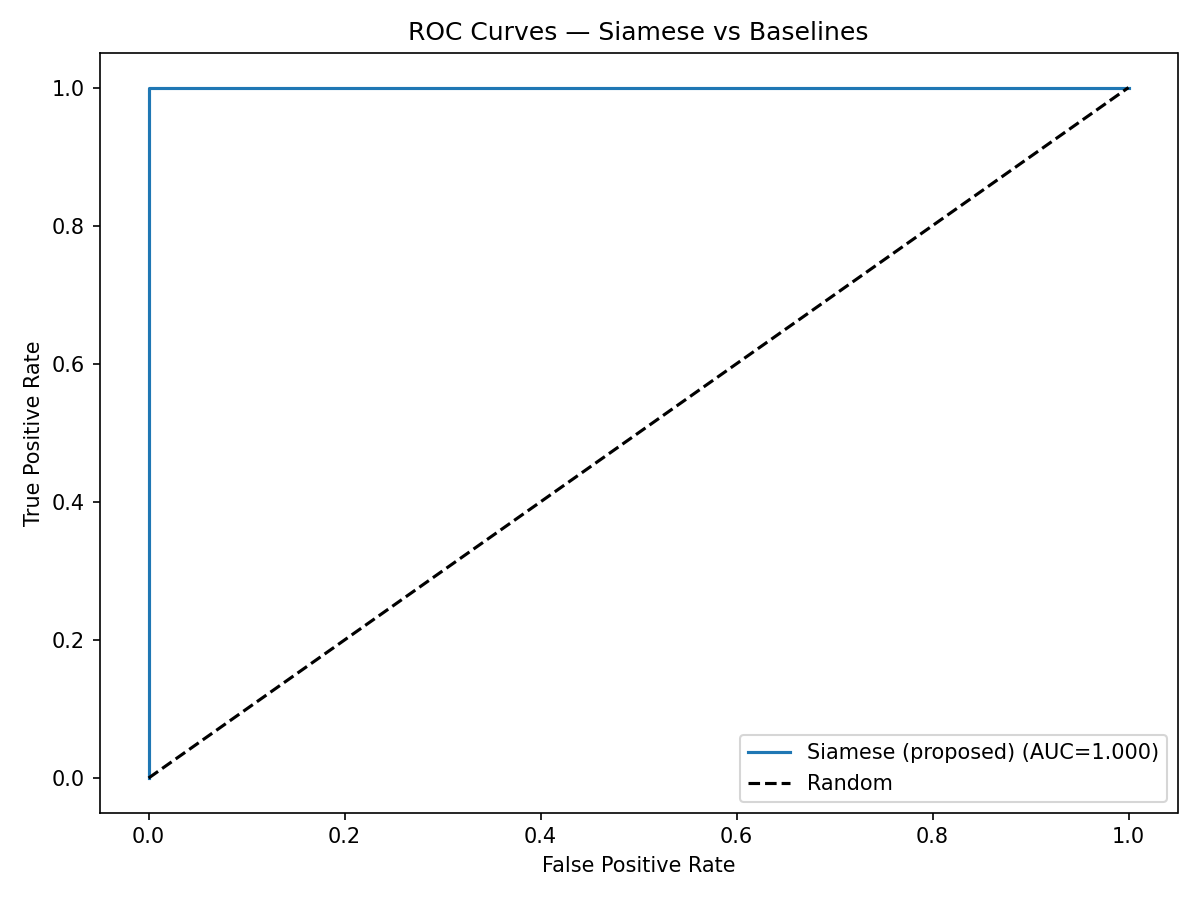
\includegraphics[width=0.9\columnwidth]{figures/roc_curves.png}
\caption{ROC curves for all three models on the held-out test set.}
\label{fig:roc}
\end{figure}

\begin{figure}[h]
\centering
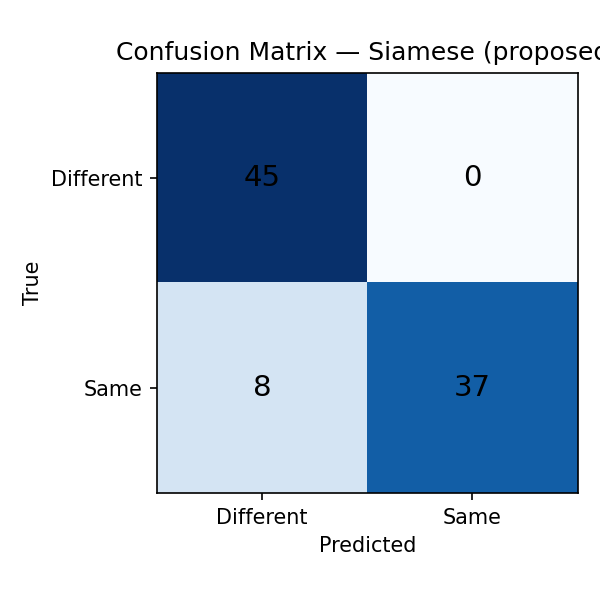
\includegraphics[width=0.7\columnwidth,keepaspectratio]{figures/cm_siamese.png}
% FIXME(caption -- write in your own words): Siamese confusion matrix on the 90-pair test set -- TN=45, FP=0, FN=8, TP=37.
\caption{[write your caption here]}
\label{fig:cm_siamese}
\end{figure}

\subsection{Autoencoder Grade-Drift Results}
% ⚠ DRAFT from companion §3.5 + §4.3 — in my voice, polish before submitting.
The autoencoder was trained only on the compliant styled images, and its
rejection threshold was set at the 95th percentile of the training
reconstruction errors ($\mathrm{MSE} = 0.00503$; training mean $0.00402$). To
test it, I distorted held-out compliant images into synthetic off-grade probes
--- hue-shift, overexposure and desaturation (Fig.~\ref{fig:gradedrift}).
Compliant images reconstruct with a mean MSE of $0.00374$, the distorted probes
with $0.00865$: more than double, which is the separation the detector relies
on. The threshold percentile is a business dial, not just a technical one --- the
90th percentile catches 62\% of drifted images at a 10\% false-alarm rate, the
95th catches 26\% at 5\%, and the 99th only 3\% at 1\%. Where to sit on that
curve is a reshoot-cost versus review-cost decision.

\begin{figure}[h]
\centering
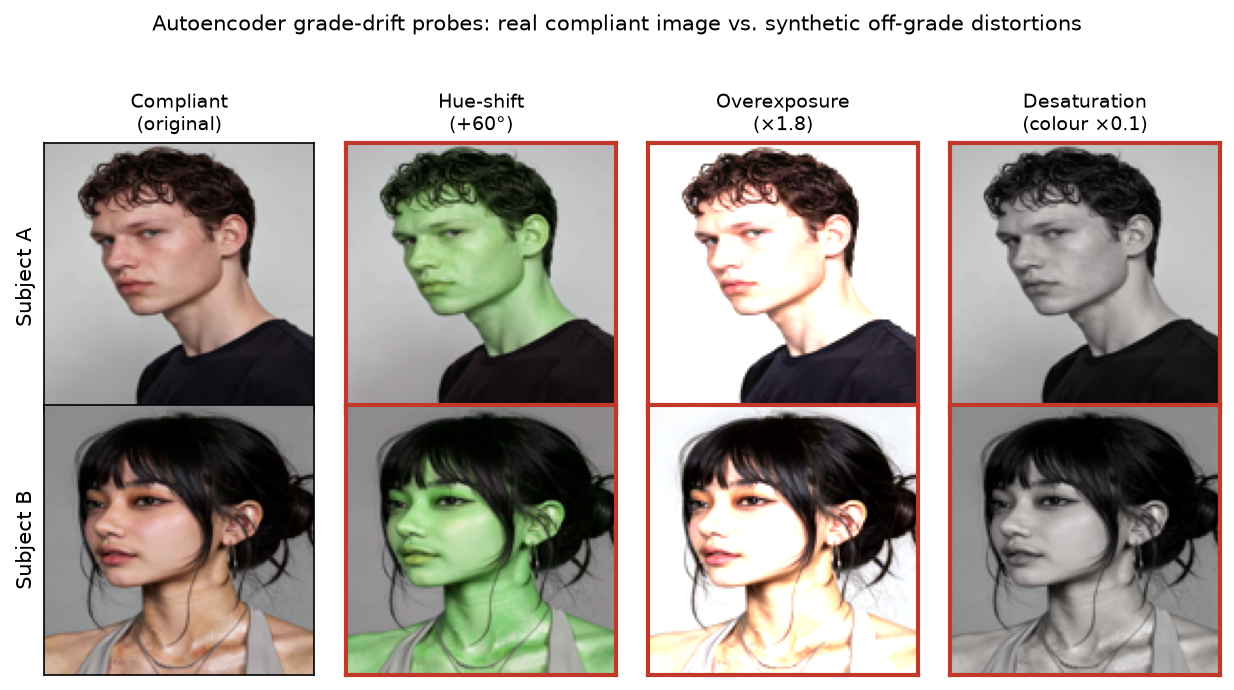
\includegraphics[width=\columnwidth,keepaspectratio]{figures/grade_drift_examples.png}
% FIXME(caption -- write in your own words): real compliant styled image vs synthetic off-grade probes (hue +60deg, brightness x1.8, colour x0.1).
\caption{[write your caption here]}
\label{fig:gradedrift}
\end{figure}

\subsection{Parametrisation Study}
% ⚠ DRAFT from companion §4.5 + §5 — in my voice, polish before submitting.
I ran four parametrisation experiments (full numbers in
\texttt{parametrisation\_experiments.json}) and five advanced ones
(\texttt{advanced\_experiments.json}); four findings stand out. (1) The single
most impactful hyperparameter was the decision threshold --- a value nobody
chose, the sigmoid default of 0.5. Tuning it on the validation set only (never
the test set) to 0.4821 recovered all 8 false negatives with zero new false
positives, lifting test $F_1$ from 0.90 to 1.0. (2) Published conventions do not
transfer blindly: the \texttt{face\_recognition} 0.6 distance rule, calibrated
on natural photos, was badly miscalibrated here --- sweeping it lifted kNN $F_1$
from 0.36 (at 0.4) to 1.0 (at 0.8). (3) Embedding dimension barely matters ---
ROC-AUC stays 1.0 at 64, 128 and 256 --- evidence that the frozen ResNet50
features, not the projection head, carry the discriminative power; I keep 128 for
comparability with FaceNet. (4) On the advanced side, the L1 head beat Euclidean
and cosine ($F_1$ 0.875 vs 0.667), a monotonic ablation ladder showed every
component earns its place (ROC-AUC $0.909$ raw pixels $\rightarrow 0.975$
embeddings $\rightarrow 1.0$ Siamese), and fine-tuning the backbone gave no gain
over freezing it, which justifies the frozen-backbone choice. Reported honestly:
McNemar's test against pixel-diff was not significant ($p = 0.19$) on only 90
test pairs --- a genuine low-power limitation.

\subsection{Error Analysis}
% REQUIRED SUBSECTION — markers look for this explicitly

\begin{figure}[h]
\centering
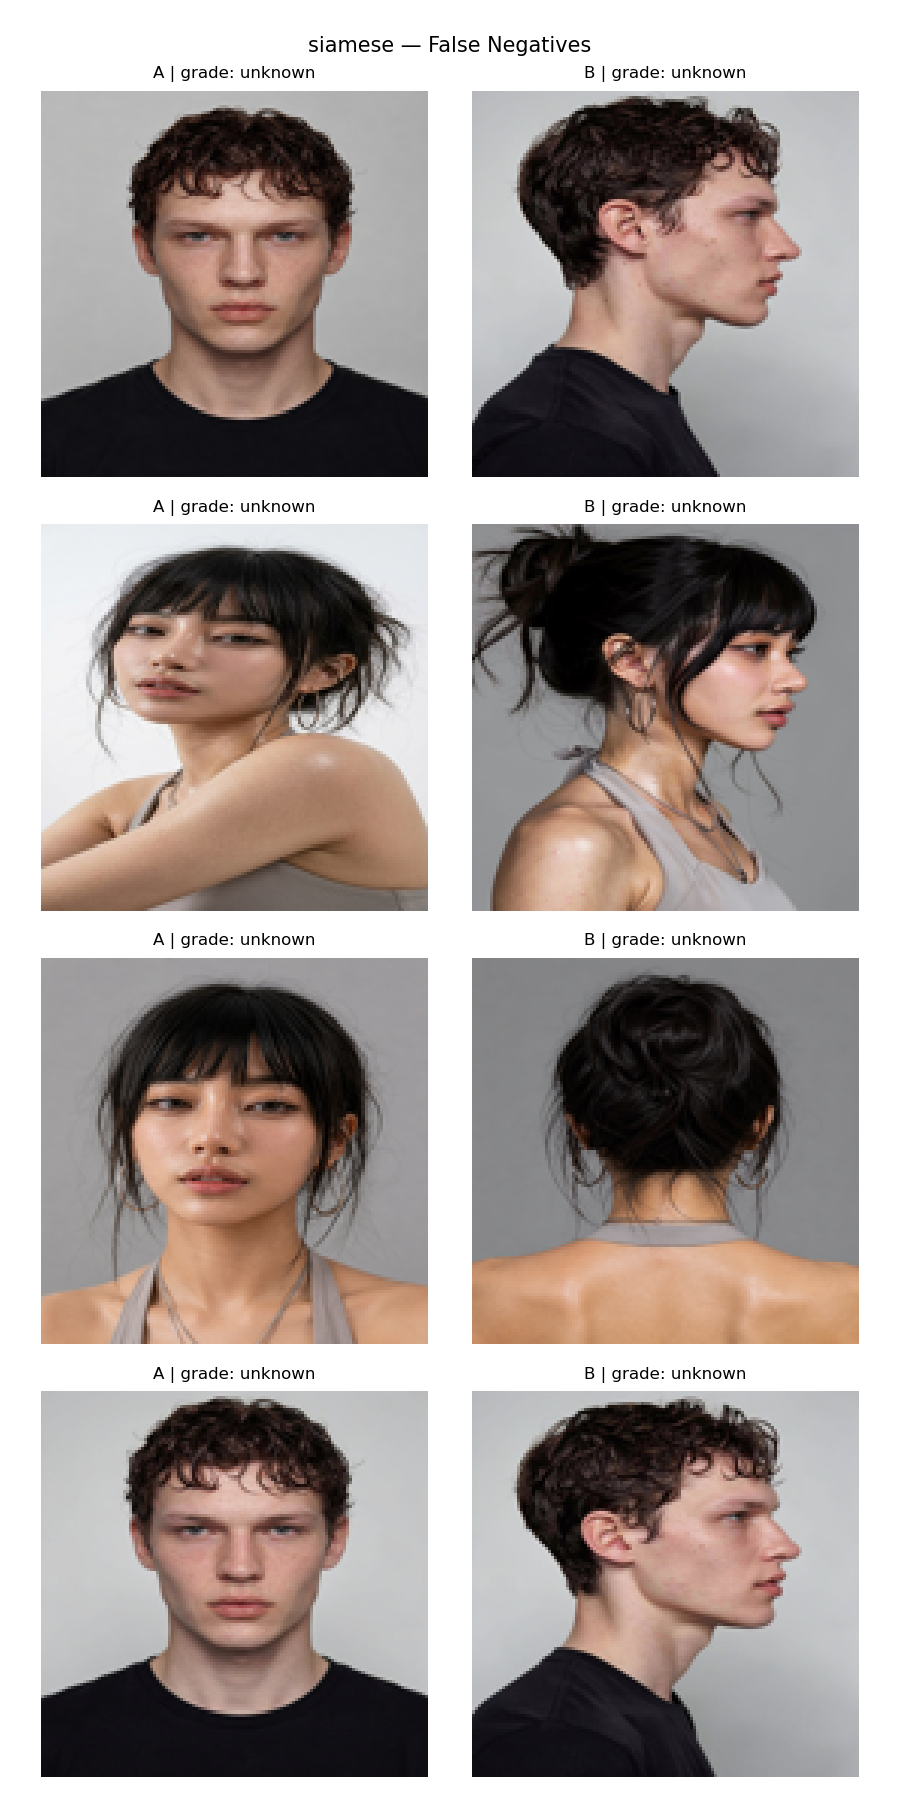
\includegraphics[width=\columnwidth,keepaspectratio]{figures/fn_siamese.png}
% FIXME(caption -- write in your own words): all 8 Siamese false negatives; every one is a same-subject pair at profile/back angles (low face-visibility).
\caption{[write your caption here]}
\label{fig:fn_siamese}
\end{figure}

% ⚠ DRAFT from companion §1.8 + §3.4 — in my voice, polish before submitting.
The system made \emph{zero} false positives and 8 false negatives on the test
set. Every false negative is a same-subject pair the Siamese scored as different,
and reading the image paths in \texttt{error\_analysis\_siamese.json} shows the
pattern: all 8 are back or profile shots --- the angles where the least face is
visible (Fig.~\ref{fig:fn_siamese}). The model was not wrong about the face; it
simply could not see enough of it. The baselines fail the same way but far
worse --- pixel-diff misses 26 and kNN misses 31 --- which confirms angular
variation is the shared hard case, not a Siamese-specific weakness.

\emph{Honest note:} the automatic grade-wise counter returned
\{\texttt{unknown}: 8\} because the pair manifest carries no grade key, so the
angle insight comes from the image paths, not from that counter. The fixes
follow directly from the failure mode --- not enough face visible: more
angle-diverse reference shots, decision-threshold tuning (already shown in the
Parametrisation study to recover all 8 misses), and harvesting extra angles from
video frames as future work.

% ============================================================
\section{Conclusions and Future Work}
\label{sec:conc}
% 5% of marks. Answer the research question directly. State limitations. 2 future directions.

% ⚠ DRAFT from companion REPORT MAP (VI. Conclusions) — in my voice, polish before submitting.
This project set out to gate AI-generated campaign images for two failures at
once, and the numbers answer the question directly: a Siamese network on frozen
ResNet50 embeddings reaches $F_1 = 0.90$ (ROC-AUC $= 1.0$, zero false positives),
against $0.59$ for pixel difference and $0.26$ for kNN --- metric learning on
frozen embeddings clearly beats raw pixel comparison for subject verification.
The autoencoder adds a second, unsupervised guard for grade drift, catching 62\%
of off-grade probes at a 10\% false-alarm rate.

The limitations are real and reported honestly: the dataset is small (106
images, 2 subjects, 90 test pairs), and with that little test data McNemar's test
could not confirm the Siamese advantage as statistically significant
($p = 0.19$) --- low statistical power, not a null result.

Future work: (1) extend the identity check to video --- frame-level Siamese
scoring of generated clips for temporal consistency (piloted privately; not part
of this submission); (2) scale the dataset by active learning, routing
low-confidence gate decisions to manual review and folding the hard cases back
into training; and (3) fine-tune the backbone on a larger synthetic-face corpus,
the one lever the ablation suggests is still untapped.

% ============================================================
\section*{References}
\bibliographystyle{IEEEtran}
\bibliography{references}

\end{document}
